\section{Evaluation Method}\label{Evaluation_Method}

For the development of our work, we used two labs. To find the probing rate to run our experiments in the remote testbed we ran tests in our In-Office lab.

\subsection*{In-Office Lab}

The In-office lab was mainly used to work on finding the probing rate to be used in the experiments at remote lab we worked with. The setup at our office is primarily composed by the following elements.

\begin{enumerate}
	\item Raspberry Pi 3 running Raspbian GNU/Linux 8 (Jessie)
	\item Wireless Access Point TP-Link AC1750
	\item Dell Laptop Inspiron running Ubuntu 16.04.4 LTS (Xenial Xerus)
\end{enumerate}

The wireless card driver on the Dell Laptop supported 802.11 a/b/g/n/ac. The driver is \textit{iwlwifi} version 4.4.0-130-generic and firmware=17.948900127.0. At the In-Office lab we setup our deployment as illustrated in figure \ref{image:In_Office_Lab_Deployment}.

\begin{figure}[h]
	\centering
	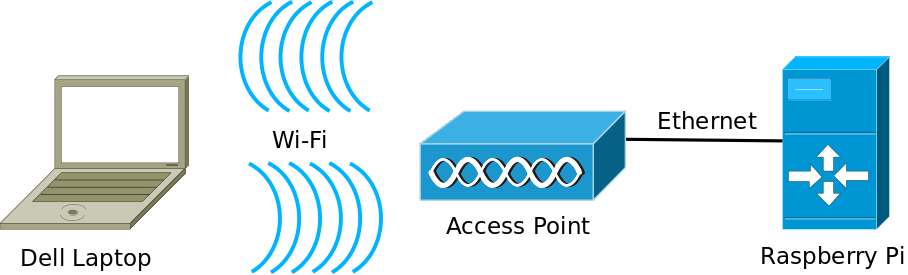
\includegraphics[width=8cm]{Deployment/In_Office_Lab}
	\caption{In-Office Lab Deployment}
	\label{image:In_Office_Lab_Deployment}
\end{figure}

The Pi was the device from which we send the pings towards the Laptop. As illustrated in figure \ref{image:In_Office_Lab_Deployment} the Pi and access point are connected via Ethernet. The laptop is connected with the AP via 802.11n. During the tests at the In-lab office we switched between 2.4 and 5.0 GHz band depending on the goal of the experiment. The In-Office lab played a key role to test the features we included in our GoPing tool prior to running experiment at the remote lab.

\subsection*{Orbit Lab}

The second testbed we work with is Orbit Lab \cite{orbit2005}. Orbit lab is a large testbed in which different Wireless technologies can be tested. One of these Wireless technologies is 802.11. Within Orbit Lab we work with Sandbox 4 (SB4) which includes features to vary the attenuation between the nodes in the Sandbox. The main components of SB4 we work with are the followings.

\begin{enumerate}
	\item SB4 has 9 nodes, each one of them runs Ubuntu 12.04
	\item Attenuation Controller which makes possible to vary the attenuation between the nodes.
\end{enumerate}

Each of the nodes has an Atheros Wireless card, the models are Atheros 5K and 9K. The nodes we work with have Atheros chipsets which allow us to collect detailed WiFi logs. The links between the nodes in SB4 can be set to attenuation values between 0-30 dBm from the attenuation controller. The topology of SB4 depends on the attenuation values for each link. For example, a full-mesh topology is achieved when the attenuation value for all the links is set to 0 dBm. Thanks to the attenuation controller we can set experiments in which changes on the RSSI are visible. The RSSI, as descried in section \ref{Wireless Monitoring Metrics}, is a metric which can help to identify attenuation impairments. The main deployment we use in  Orbit is similar to the deployment we have at the In-office lab. The node working as AP was setup using the \emph{hostapd} utility. The WLAN settings for the AP are summarized in table \ref{table:WLAN_Settings_AP_Node}.

\begin{table}[h]
	\begin{center}
		\begin{tabular}{||c c||}
			\hline
			Setting & Value\\ [0.5ex] 
			\hline\hline
			802.11 Protocol & 802.11n\\ 
			\hline
			Channel Bonding & No\\
			\hline
			Band & 2.4 GHz\\
			\hline
			Security & Open\\ [1ex] 
			\hline
		\end{tabular}
	\end{center}
\caption{WLAN Settings at AP Node}
\label{table:WLAN_Settings_AP_Node}
\end{table} 


\subsection*{Experiments Setup}

To trigger WiFi and non-WiFi impairments we setup three main scenarios in Orbit SB4 testbed. Two of them, attenuation and congestion, are WiFi-related. The third one is an access link impairment. Across the three scenarios we let running the collection of active and passive measurements. Our experiment sessions last 10 min. Passive wireless metrics logs are collected every 10 secs at the AP and Wireless client. We also setup a Wireless a Sniffer to obtain Over-the-Air packet captures. From the wired client we send pings towards the AP and log the stats from GoPing. For the throughput measurement with iPerf, we setup iPerf server at the wireless node and the iPerf client at the wired node. iPerf was setup in TCP mode with 4 parallel TCP streams. We chose TCP as it is transport protocol most commonly used by services at Home WiFi networks. We work with 4 parallel streams as within the Home WiFi the number of TCP streams is average below 5 \textbf{[We need a reference here]}.

\subsection*{Attenuation}

To trigger attenuation impairments in the testbed we vary the attenuation at the link between the wireless client and the access point. As mentioned before the setup we use at SB4 in Orbit is similar to our In-Office lab which is illustrated in figure \ref{image:In_Office_Lab_Deployment}. The additional component to this setup is the node working as a wireless sniffer. The attenuation impairment happens in the 3\textsuperscript{rd} and 9\textsuperscript{th} minute of the 10 min session. The experiment is designed this way to set a comparison between impairment-free and impairment conditions. We setup 5 scenarios with an increase of 3 dBm per impairment interval. Table \ref{table:Attenuation_Experiment_Values} breakdowns the scenarios and the attenuation levels for each impairment interval. We ran each experiment 5 times.

\begin{table}[h!]
	\begin{center}
		\begin{tabular}{|| m{5em} | m{2cm}| m{2cm} ||}
			\hline
			\multirow{2}{*}{Scenario} & \multicolumn{2}{c||}{Attenuation Value {[}dBm{]}} \\ \cline{2-3} 
			& \multicolumn{1}{l|}{1st Interval} & \multicolumn{1}{l||}{2nd Interval} \\ \hline\hline
			1 & 3 & 6 \\ \hline
			2 & 9 & 12 \\ \hline
			3 & 15 & 18 \\ \hline
			4 & 21 & 24 \\ \hline
			5 & 27 & 30 \\ \hline
		\end{tabular}
	\end{center}
	\caption{Attenuation Scenarios and Values}
	\label{table:Attenuation_Experiment_Values}
\end{table}

\subsection*{Congestion}

To trigger congestion in our testbed, we connect more wireless clients to the same AP our main wireless client is connecting to. At the 4\textsuperscript{th} and 8\textsuperscript{th} minute we connect an additional wireless clients to the AP. The additional wireless clients send UDP traffic to the AP using iPerf, hence the AP is running an iPerf server instance. We increase by one the wireless nodes connecting to the AP per interval. Table \ref{table:Congestion_Experiment_Values} consolidates the scenarios and number of wireless nodes connecting to the AP per interval.

\begin{table}[h!]
	\begin{center}
		\begin{tabular}{|| m{5em} | m{2cm}| m{2cm} ||}
			\hline
			\multirow{2}{*}{Scenario} & \multicolumn{2}{l||}{Connected Wireless Nodes} \\ \cline{2-3} 
			& \multicolumn{1}{l|}{1st Interval} & \multicolumn{1}{l||}{2nd Interval} \\ \hline\hline
			1 & 1 & 1 \\ \hline
			2 & 2 & 2 \\ \hline
			3 & 3 & 3 \\ \hline
			4 & 4 & 4 \\ \hline
			5 & 5 & 5 \\ \hline
		\end{tabular}
	\end{center}
	\caption{Congestion Scenarios and Values}
	\label{table:Congestion_Experiment_Values}
\end{table}

\subsection*{Access Link Limiting}

The third scenario triggers a non-WiFi impairment. The experiment consists in limiting the access link capacity at the Wired node. We achieve limiting at the wired node by using \emph{tc}, a traffic shaper utility. In a similar way to the attenuation scenario, we trigger the impairment conditions at the 3\textsuperscript{rd} and 9\textsuperscript{th} minute of the 10 min experiment window. Table \ref{table:Access_Link_Experiment_Values} details the scenarios and values for the Access Link Limiting scenario.

\begin{table}[h!]
	\begin{center}
		\begin{tabular}{|| m{5em} | m{2cm}| m{2cm} ||}
			\hline
			\multirow{2}{*}{Scenario} & \multicolumn{2}{c||}{Throughput {[}Mbps{]}} \\ \cline{2-3} 
			& \multicolumn{1}{l|}{1st Interval} & \multicolumn{1}{l||}{2nd Interval} \\ \hline\hline
			1 & 100 & 90 \\ \hline
			2 & 80 & 70 \\ \hline
			3 & 60 & 50 \\ \hline
			4 & 40 & 30 \\ \hline
			5 & 20 & 10 \\ \hline
		\end{tabular}
	\end{center}
	\caption{Access Link Limiting Scenarios and Values}
	\label{table:Access_Link_Experiment_Values}
\end{table}

\subsection{RSSI in the wild}

With regards to the attenuation scenario we ran a survey to find the common RSSI value in home and office environments. We asked the colleagues at our office to run a script which collects WiFi metrics on their laptops at different times during their stay at home or office. From the 760 samples collected we found that the most common RSSI value ranges between -60 and -65 dBm. Figure \ref{fig:RSSI_Histogram} illustrates the RSSI histogram of our survey.

\begin{figure}[h]
	\centering
	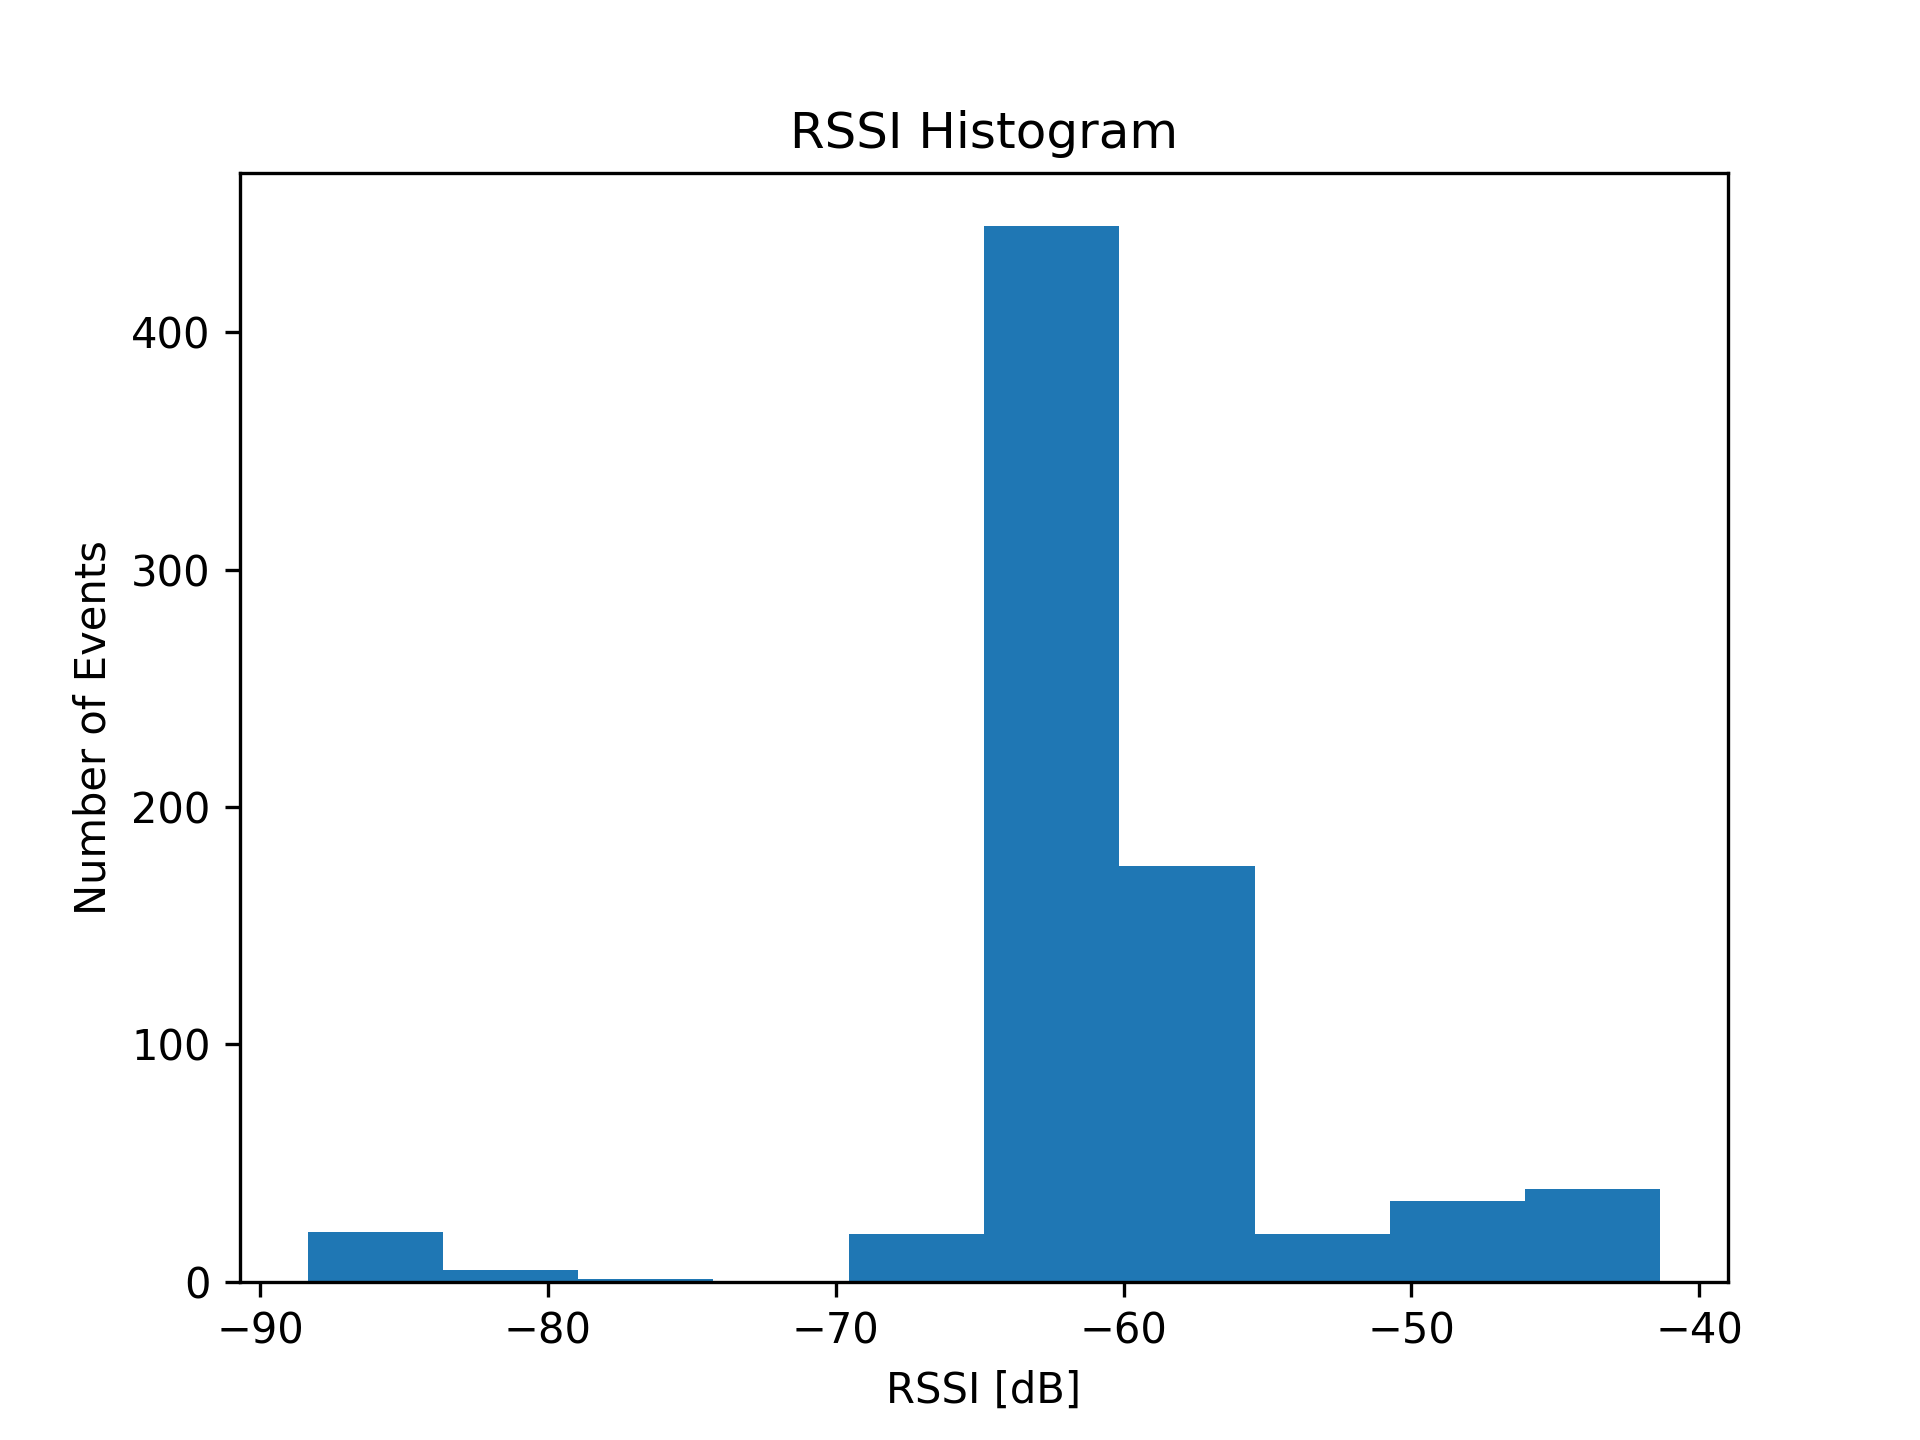
\includegraphics[width=8cm]{RSSI_Stats/RSSI_Histogram}
	\caption{RSSI Survey Values Histogram}
	\label{fig:RSSI_Histogram}
\end{figure}

The main goal of this exercise was to validate attenuation values to be used for our experiments. In Orbit SB4 testbed, attenuation values of 0, 3 and 6 [dBm] led to RSSI values between -60 and -65 dBm, which is the range obtained from our survey. These values are included in the attenuation experiments we ran.



